\documentclass[12pt]{article}
\usepackage[utf8]{inputenc}
\usepackage{hyperref}
\usepackage{graphicx}
\usepackage{float}
\usepackage{xcolor}
%Insert tab
\providecommand{\tab}{\hspace{10pt}}
\title{SPIFI Improvements Report}
\author{Brennan W. Fieck}
\begin{document}
\begin{titlepage}
\clearpage\maketitle
\thispagestyle{empty}
\begin{figure}[H]
\centering

\includegraphics[width=0.5\textwidth]{team-logo.png}
\end{figure}
\end{titlepage}

\section*{Introduction}
The basis of the broader project to which this team's efforts contribute
is to expand upon an existing technology called  Spatial Frequency
Modulated Single Detector Imaging (SPIFI). This team created simulation
software and measurement software dealing with potential improvements to
the SPIFI technique. The simulation served as a proof-of-concept as well
as a helpful guide for what has come to be known as "2D-SPIFI". The measurement software is used to implement photon-counting rather than conventional detection methods.

\section*{Background}
SPIFI is a revolutionary imaging technique that allows a line to be scanned
across an object by a single laser at one time, without using a raster pattern
along the line. This represents a performance change from $O[n^2]$ to $O[n]$ for a square object with side length $n$. SPIFI accomplishes this by encoding the information about an object in a
frequency change which maps directly to a spatial line that spans the object,
and which evolves in time as the line sweeps over the object. Traditionally, scanning more than a single point at a time
would require multiple collectors to be able to
resolve which photons were used to scan what part of the object (e.g.
using a camera). Figure \ref{fig:cube-line} depicts part of a very simple SPIFI system being used to image a gray cube.

\begin{figure}[ht]
	\centering
	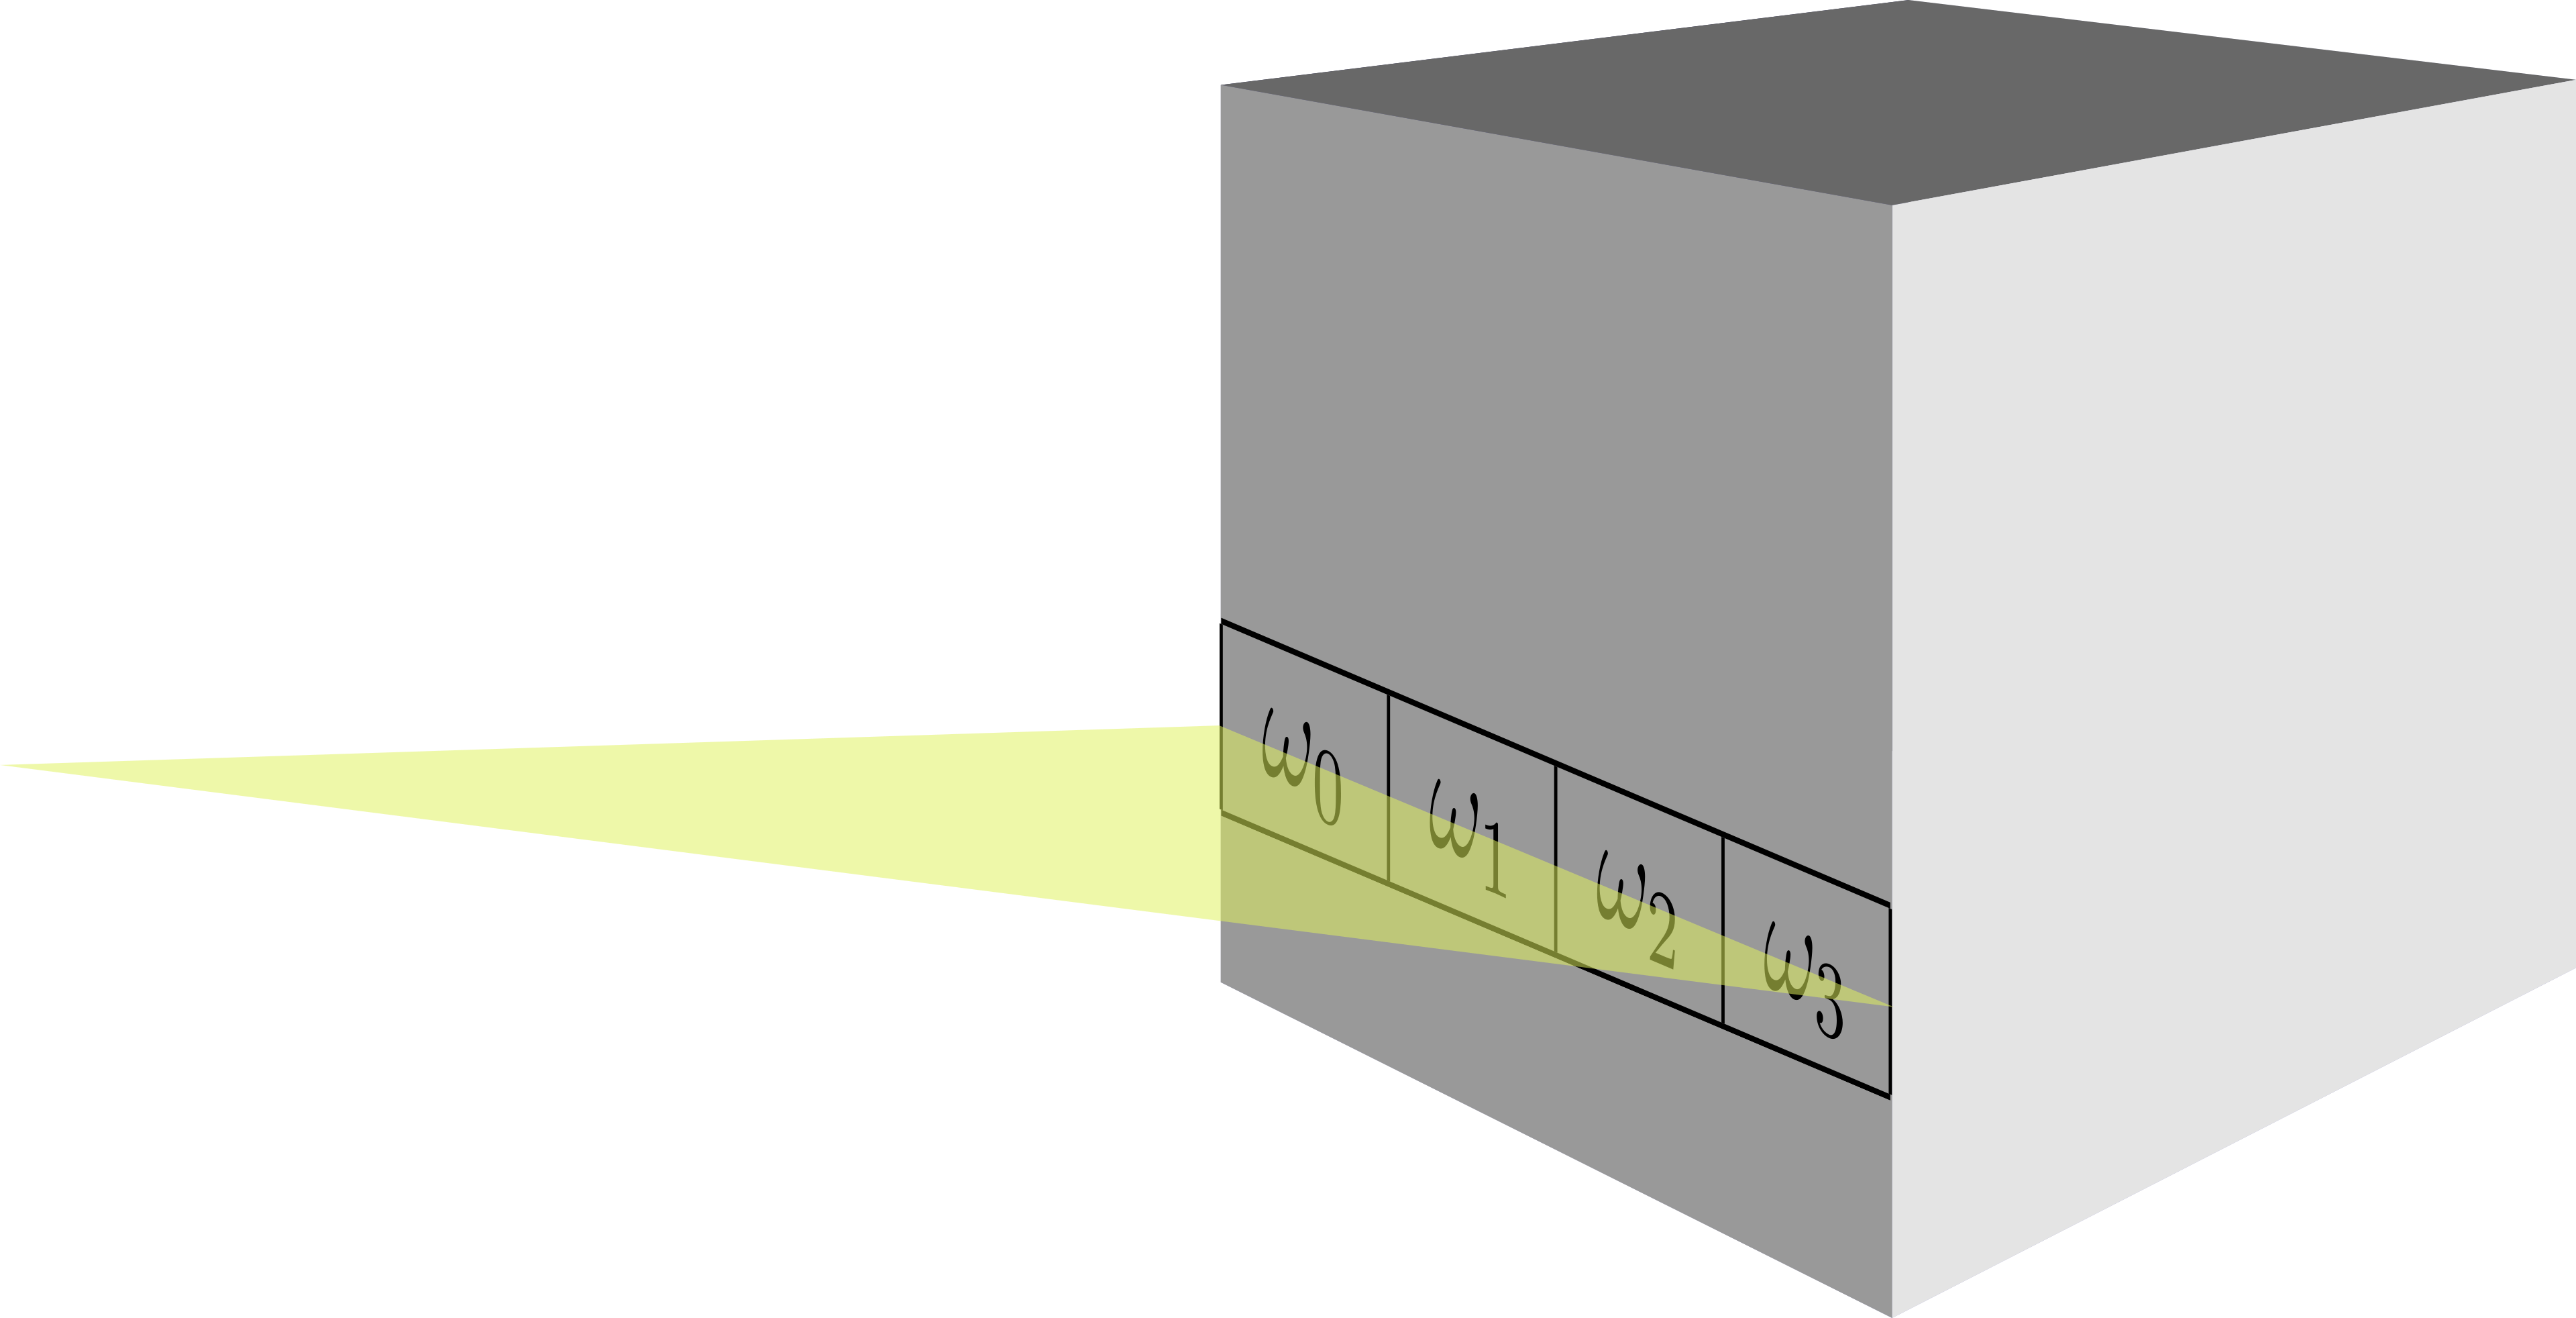
\includegraphics[width=0.75\textwidth]{spifi-line-on-cube.png}
	\caption{Visual Depiction of Spatial Frequency Mapping}
	\label{fig:cube-line}
\end{figure}

The four $\omega$s in boxes represent different, unique frequencies along the plane of light hitting the object. Of course, in practice the frequency modulation is smoother and the resolution of the imaging is determined by how many "boxes" one can make on the face of the object. The sheet of light is mechanically swept across the object, and as it moves the frequencies each evolve at different rates. Figure \ref{fig:cube-sheet} shows how frequency varies in time as the sheet of light sweeps over the object.

\begin{figure}[ht]
	\centering
	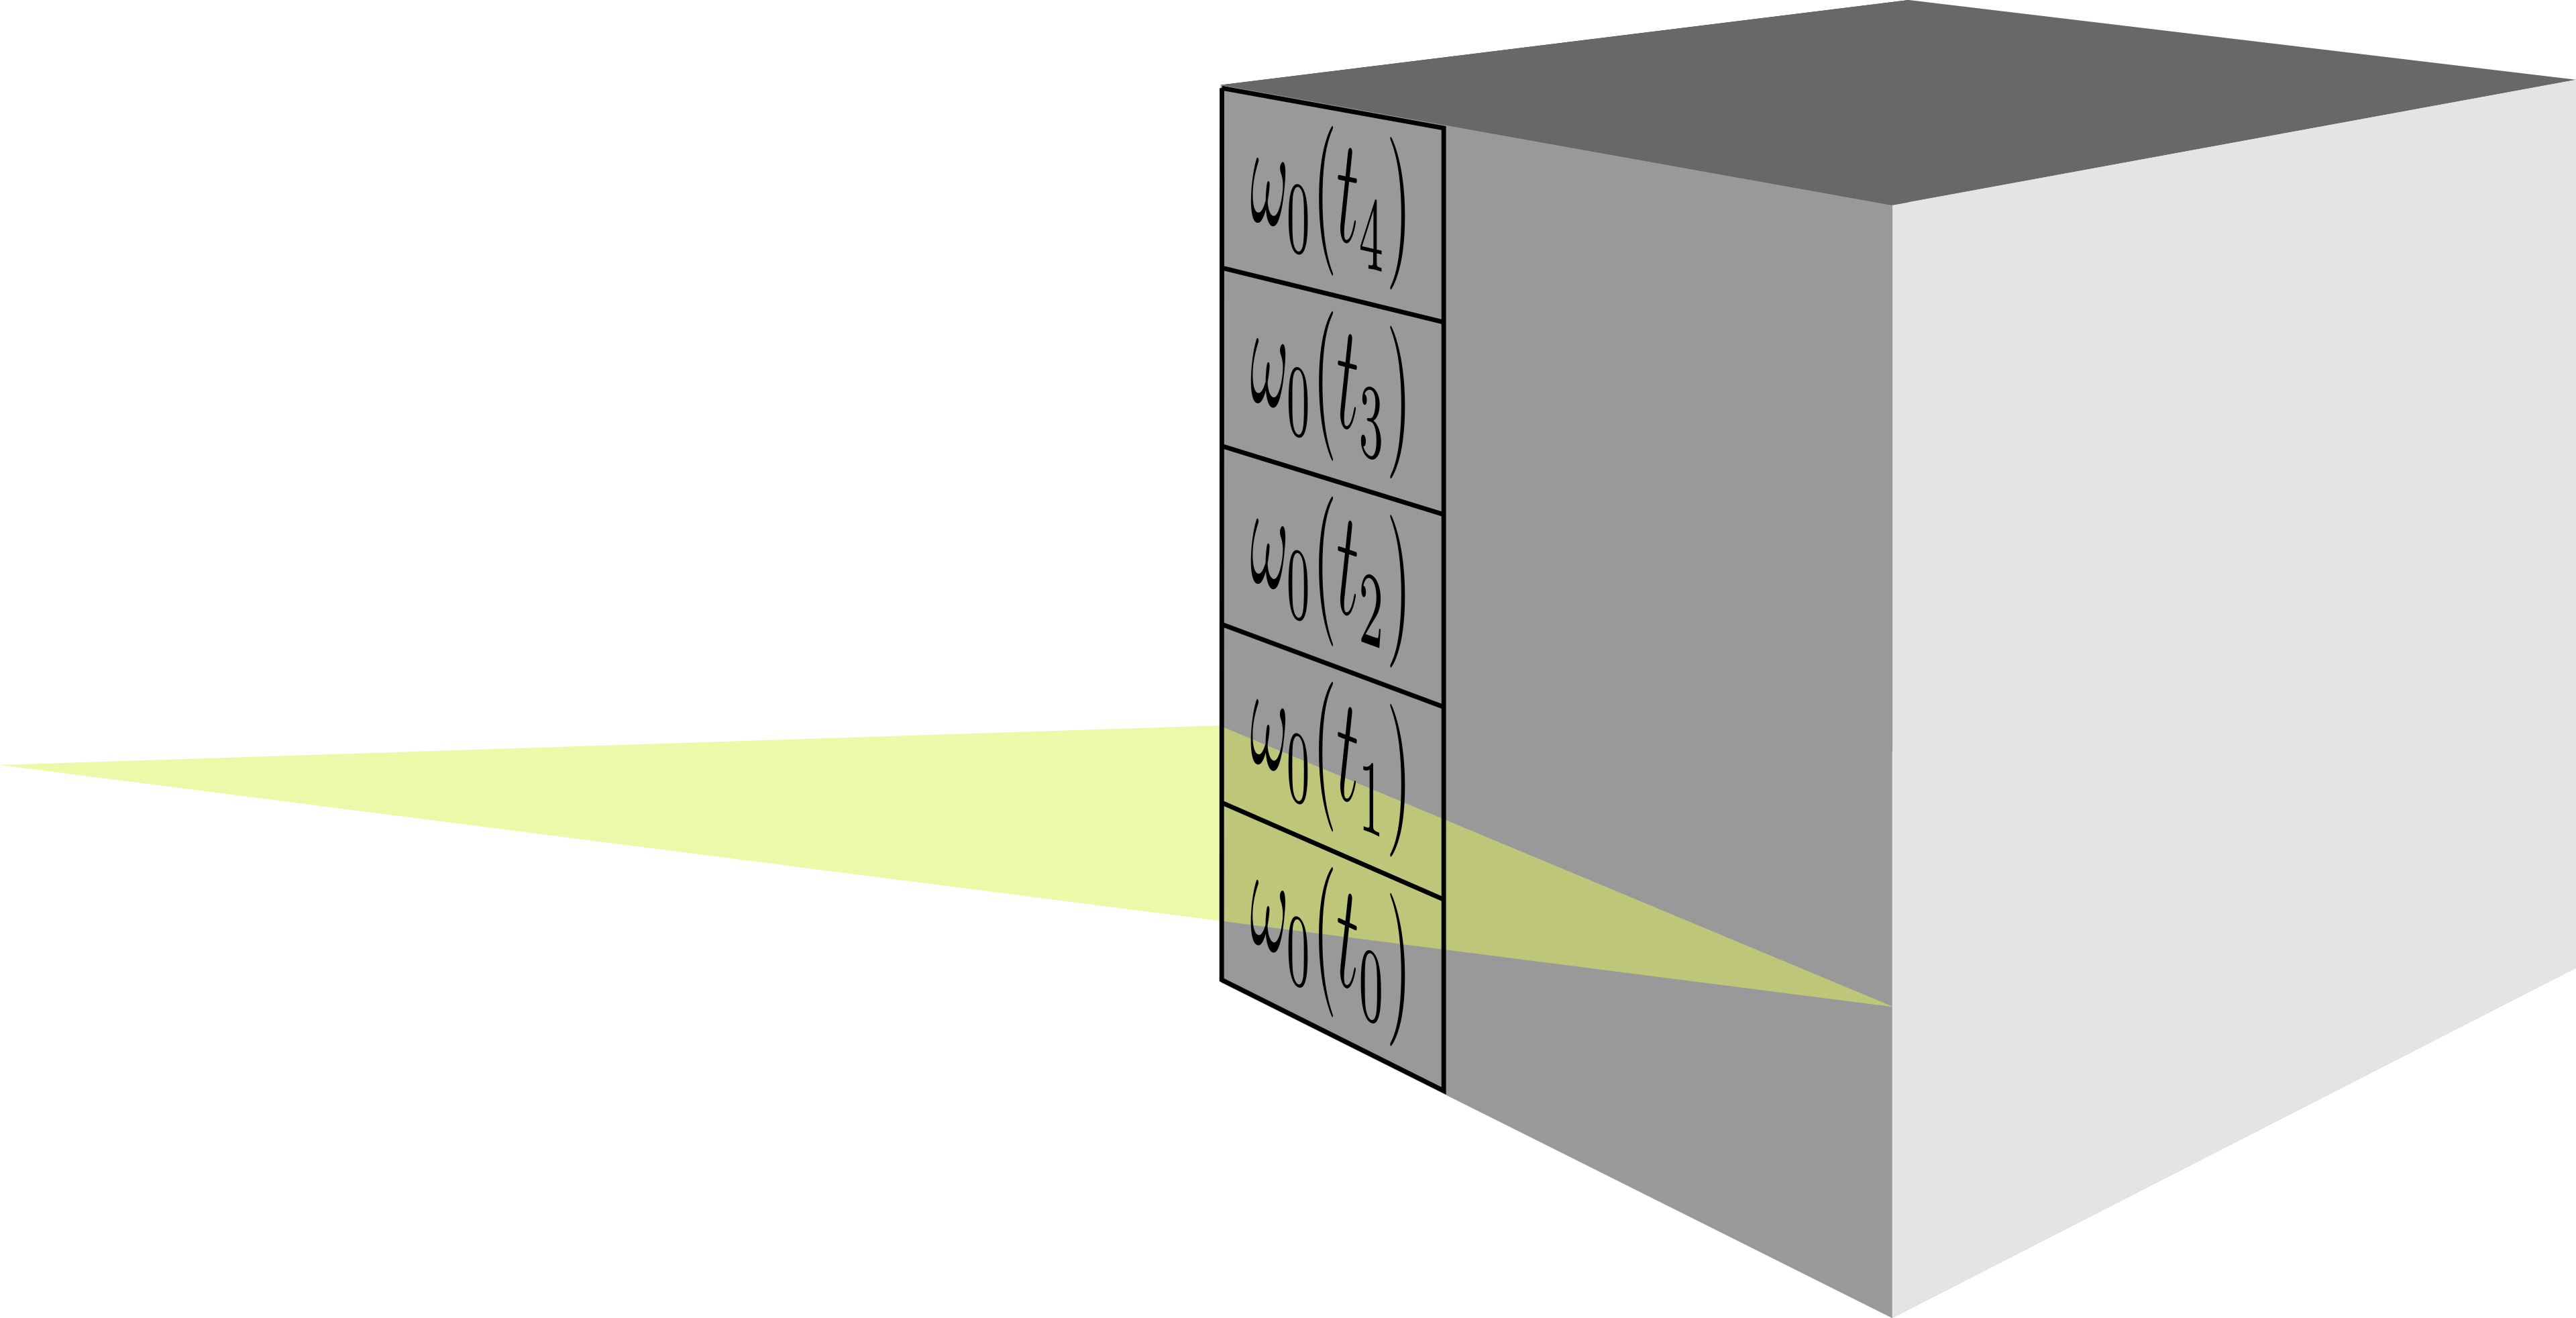
\includegraphics[width=0.75\textwidth]{spifi-sheet-on-cube}
	\caption{Visual Depiction of Temporal Frequency Mapping}
	\label{fig:cube-sheet}
\end{figure}



\begin{figure}[ht]
\centering
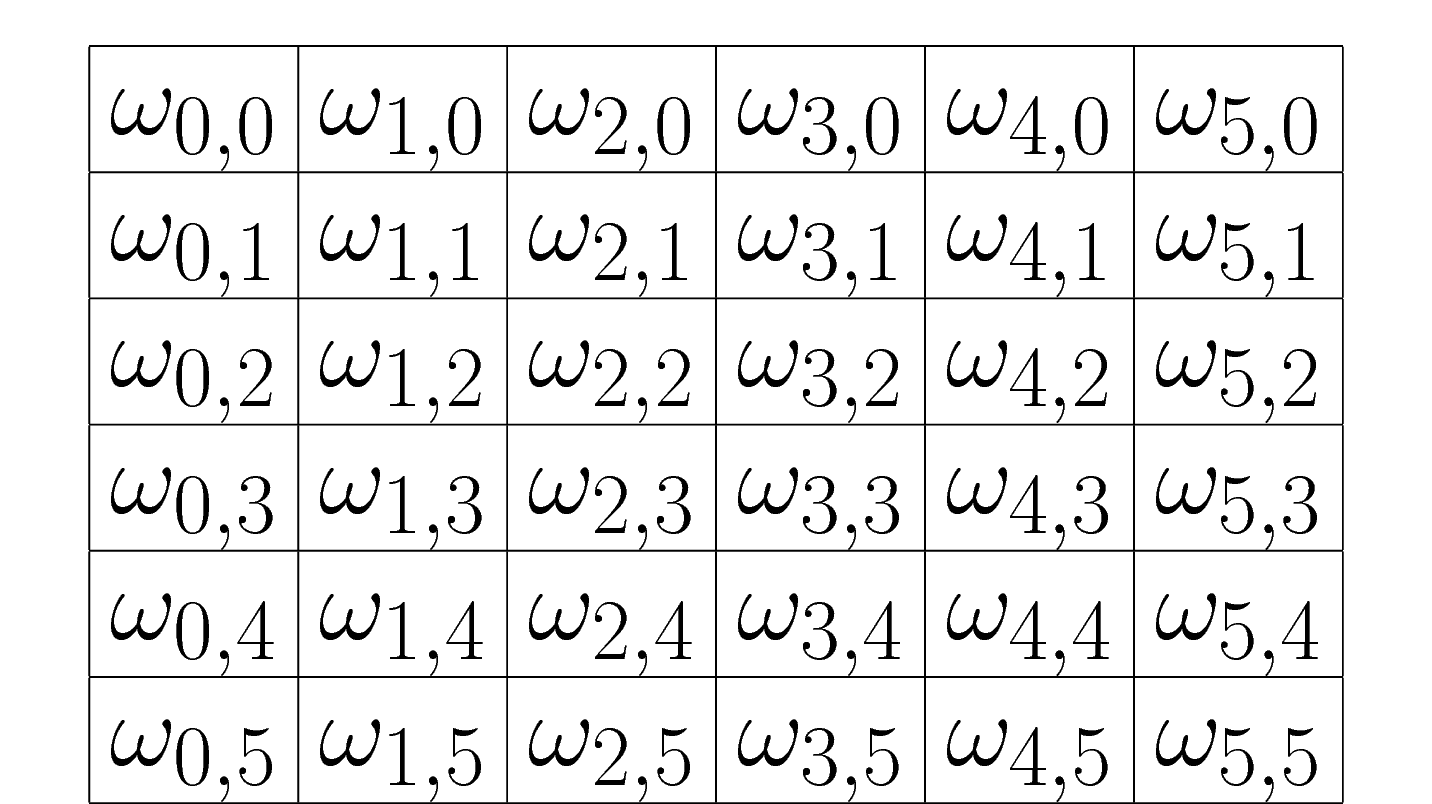
\includegraphics[width=0.75\textwidth]{spifi-grid.png}
\caption{Total Frequency Mapping Over an Object\label{fig:mapping-diagram}}
\end{figure}

Figure \ref{fig:mapping-diagram} shows the net result of these temporal and spacial frequency mappings;
each inscribed $\omega$ is unique to the section of the
$x/y$ plane that bounds it. After passing through the object, the light is gathered back into a well-collimated beam and collected by a single-pixel detector. Then decomposing the measured signal into the frequencies that make it up allows for inspection of how the laser interacted with the object at specific points on its surface. Each of these tiny "boxes" as seen in Figure \ref{fig:mapping-diagram} can be interpreted directly as a pixel. This is done by measuring the attenuation of the specific frequency. For example, considering once again Figure \ref{fig:mapping-diagram}, suppose that the measured signal has almost none of the frequency $\omega_{2,2}$ in it, but has nearly all of the $\omega_{0,0}$ that it started with. This means that light in the upper-left corner of the object faced almost no resistance, while nearly all of that which traveled through $(x,y)=(2,2)$ was blocked. It's then reasonable to conclude that the object is shaped such that it is relatively thick at $(2,2)$, and relatively thin at $(0,0)$.

% \begin{figure}[ht]
% \centering
% 
\includegraphics[width=0.75\textwidth]{spifi-system}
% \caption{A Simple SPIFI System Setup\label{fig:spifi-sys}}
% \end{figure}

This frequency mapping is achieved by spreading the laser into a sheet and then passing it through a SPIFI mask. Designs of these masks vary, but they can all be understood in the same manner through their transfer function acting on the laser. Figure \ref{fig:spifi-sys} shows the signal transfer system, starting with some laser given by $u(x)$. The modulation function shown, $m(x,t)$, is then applied, followed by the laser passing through the object which itself applies some unkown transfer function $g(x)$. The final result measured on the detector is an intensity, so only the square of the signal is observable.

\begin{figure}[ht]
\centering
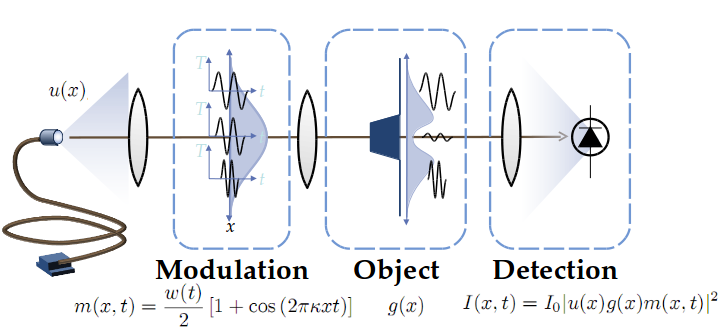
\includegraphics[width=0.75\textwidth]{spifi-system-graphical}
\caption{A Simple SPIFI System}
\label{fig:spif-sys}
\end{figure}
The transfer function $g[x,y]$ is determined
by the object being
imaged, and represents an attenuation of amplitude of specific sections of the
$xy$ plane based on the object's ability to absorb and reflect light.
Typically this function is used to describe the object, and once found will immediately yield an image of the object.

\begin{figure}[H]

\includegraphics[width=0.4\textwidth]{spinner}
\hfill

\includegraphics[width=0.4\textwidth]{rectangular_spifi_mask}
\caption{Left: A Circular SPIFI Mask -
Right: A Rectangular SPIFI Mask\label{fig:ex-grat}}
\end{figure}

Examples of typical SPIFI masks are
shown in Figure \ref{fig:ex-grat}. For the common circular grating - 
similar to the one in the figure - the form of the pattern in polar
coordinates is
\begin{equation}
\textnormal{pattern}[r,t]=\frac{1}{2}+\frac{1}{2}\cos\left[2\pi
f_mk_prt\right].
\label{eq:pattern}
\end{equation}

Here, $f_m$ is the rotational of the grating, and $k_p$ is a constant
that has to do with the density of the lines in the pattern.

\begin{figure}[H]
\centering
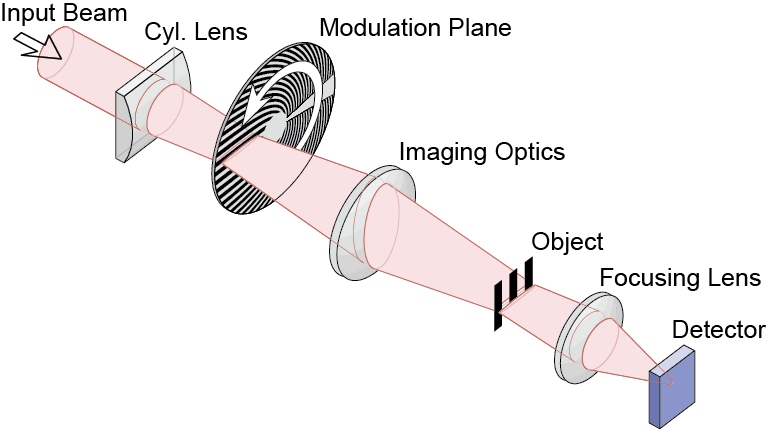
\includegraphics[width=0.75\textwidth]{circular_SPIFI_system}
\caption{A Simple SPIFI System Using a Circular Mask}
\label{fig:circ-sys}
\end{figure}

As shown in Figure \ref{fig:circ-sys}, this function modulates the laser as it passes
through the grating as a line, and then is scanned along the object from top
to bottom by a mechanical apparatus twisting a lens or mirror. A transformation from Equation
\ref{eq:pattern} to the $m[x,y,t]$ transfer function requires sampling the
output in intervals of $\tau_m=1/f_m$, the period of the pattern's 
spinning. 

Once the light has been scanned over the object, the intensity recorded by
the detector during $\tau_m$ can be Fourier-transformed to find the
contributions from each frequency at a given time. The time-domain and frequency-domain plots of this for some
unknown object looks like Figure \ref{fig:fourier}. 

\begin{figure}[H]
\centering
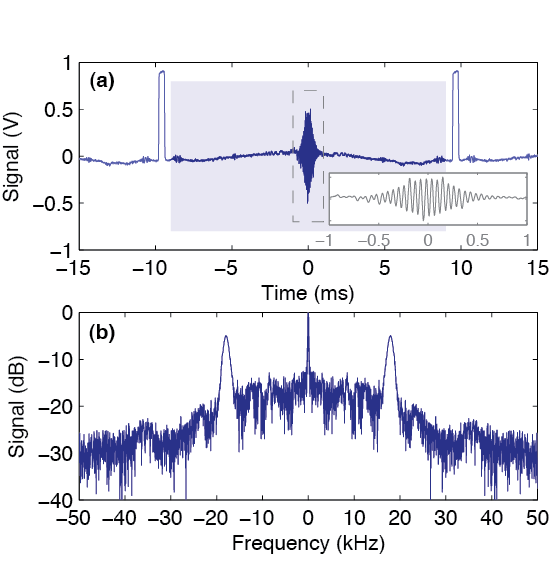
\includegraphics[width=0.75\textwidth]{Fourier_Transform}
\caption{Top: Time-Domain SPIFI Output - Bottom: Corresponding Frequency-Domain SPIFI Output\label{fig:fourier}}
\end{figure}

\section*{Theory of 2D SPIFI}
One focus of this project was to expand the capabilities of SPIFI by using a
mask which diffracts the entire beam in two dimensions at any one time,
thereby eliminating the need to mechanically scan the laser along the object. 2D-SPIFI can scan an object in constant, or $O[1]$ time, as opposed to the current technique which has a complexity of $O[n]$ where $n$ is the size of the object - and again all of this is compared to $O[n^2]$ when using traditional raster-scan techniques. This technology is still in its infancy, but if it proves reliable wil obviously vastly improve real-time imaging. As a proof-of-concept, as well as to aid in the design of 2D SPIFI masks, the team produced software capable of simulating 2D-SPIFI for more or less arbitrary objects and masks.

\begin{figure}[ht]
	\centering
	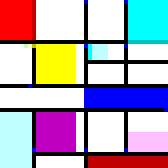
\includegraphics[width=0.45\textwidth]{testimg}
	\hfill
	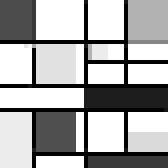
\includegraphics[width=0.45\textwidth]{testoutput}
	\caption{Left: Simulation Input "Object" - Right: Simulation Output Image}
	\label{fig:sim-in-out}
\end{figure}

Figure \ref{fig:sim-in-out} shows the input and output of the simulation when run using an image file as a representation of the object.

\section*{Photon Counting}
Previously, SPIFI measurements were taken using National Instruments$^\textnormal{\small TM}$ (NI) devices and passed through NI's proprietary LabView software for analysis. With the improved scanning speed expected from implementations of 2D-SPIFI, it will be necessary to increase processing of collected data as well. If one were able to count the photons incident on the detector, it would eliminate the need to perform Fourier transforms on the input. The energy of the photon will show up in the detection method  and therefore automatically carry the information about its frequency; e.g. photo-multiplier tubes produce current proportional to detected photon energy. So the mapping information is there and the image can begin being constructed immediately, each detected photon can be immediately added to a real-time image without the need for further computation. The computation is simple enough to be carried out efficiently by a micro-controller, so a program was devised for a Field-Programmable Gate Array (FPGA) as a first step in moving towards a headless data store. The design is fairly simple, it works by taking only two signals as inputs on the general-purpose I/O pins on the DEO-Nano FPGA. One is a reading of the laser control itself, which tells the FPGA when the laser fires a burst of photons, so that it can count them for that time period. The other input comes from the photo-multiplier tube that served as the detector. Then all the FPGA does is print a list of photons it counts during each laser pulse back through a usb cable to a normal computer. Figure \ref{fig:timing} shows an example of these signals, with the counting periods indicated.

\begin{figure}[ht]
	\centering
	\includegraphics[width=0.7\textwidth]{timing}
	\caption{Sample FPGA Input Timing Diagram}
	\label{fig:timing}
\end{figure}


\section*{Software and Licensing}
Unfortunately, the source code cannot be included here, as the research is still pending publication. At the time of publication, the source will be made available to the community along with its respective documentation.
Once released, the software is provided under the GNU Public License version 3. The simulation is written in the open Python 3.5.2 standard, with a list of free and open source dependencies that will be made available at the same time as the simulation itself. The FPGA code was written using the Quartus software which is the property of Altera$^\textnormal{\small TM}$, along with various pieces of supporting software each of which is subject to its own license. 


Firstly, the simulation will be built up in the following steps:
\begin{enumerate}
\item Simulate 2D SPIFI using a perfectly continuous grating wheel
\item Incorporate gaps between patterns on the wheel
\item Incorporate refraction and diffraction caused by equipment
\end{enumerate}
Documentation for this program will be made available in exhaustive pdf 
form as well as POSIX-compliant manual pages for the first incarnation, and
subsequently updated for each change. The program will be written in an
open language standard (C) using a free and open runtime for that 
language (the GNU Standard C library, compiled using the GNU C Compiler),
and will be written and run on existing computers.

Secondly, data collection software will be written in the following two
steps:
\begin{enumerate}
\item Analysis of existing codebase
\item Development of actual software
\end{enumerate}
Data collection software already exists for simple, 1-dimensional SPIFI
systems, so it may be advantageous to build the 2-dimensional analysis tool
by writing a new version of this suite, or even to simply add it directly
into the existing structure. Alternatively, if the current software is
found to be devoid of functionality that can be used for the new system, or
if it is deemed too bloated, slow, or incapable of interfacing properly
with the detection hardware in some way, it would be more prudent to begin
a new program and build it from the ground up. To determine which is
better, the existing code will be analyzed, ideally in
collaboration with the original team that wrote it - a coalition of
researchers and research assistants from the Colorado School of Mines and
the University of Colorado in Fort Collins, with the latter currently in
charge of maintaining and updating. After the analysis, the actual code
will have to be written. Whatever decision is reached regarding the use of
the 1-dimensional analysis software, the final product \emph{will} be
written in an open language standard, and utilize a free and open
runtime (the existing software has equivalent versions written in
C++ and C\#, so it's impossible to say exactly what language and runtime
will be used until the analysis is conducted, or even which will be used
given that the existing software is used in some capacity). However, the
current software is packaged as "Solutions" for the Microsoft IDE and
Development Environment called Visual Studio. Therefore, even if neither of
these codebases is used, Visual Studio must be used in their analysis. Not
only is Visual Studio itself not free, it only runs on the proprietary
operating system Windows version 7 or higher. Furthermore, the company Jet
Brains produces a proprietary plugin for Visual Studio that makes working
with C\# so much easier, and consequentially saves developers so much time
that the vast majority of companies that work with C\# deem it worth the
cost. Given this usefulness, and the fact that the head software engineer is already
familiar with the plugin, it would be very difficult to complete the
analysis of the existing data collection software inside of the estimated
timeframe - certainly not with the 10 h/week estimate - without the use
of the plugin.

\section*{Statement of Work}
A breakdown of the costs of completing each part of the project
is given in Table \ref{tbl:cost}, and
a timeline given for these tasks and their various parts, as well as the
report to be presented on completion is given in Table \ref{tbl:time} and
the data is visualized in Chart \ref{chrt:time}.

\begin{table}[h]
\centering
\begin{tabular}{l|r|c|c|r}
\bf{Item} & \bf{Unit Cost} & \bf{Quantity} & \bf{Unit} & \bf{Cost}\\
\hline
2D Simulation Software & & & & \\
\tab$\cdot$ Labor & \$63.00 & 28 & day & \$1764.00\\
\hline
Data Collection Suite & & & & \$6401.00\\
\tab$\cdot$ Labor & \$63.00 & 87 & day & \$5481.00\\
\tab$\cdot$ Visual Studio License & \$500.00 & 1 & ea & \$500.00\\
\tab$\cdot$ Windows 10 Product License & \$120.00 & 1 & ea & \$120.00\\
\tab$\cdot$ JetBrains Resharper License & \$300.00 & 1 & ea & \$300.00\\
\hline
Final Report & & & & \\
\tab$\cdot$ Labor & \$63.00 & 36 & day & \$2268.00\\
\hline
\tab$\cdot$ Overhead & 50\% of Labor & -- & -- & \$4756.50\\
\hline
\bf{Total Cost} & & & & \bf{\$15,189.00}
\end{tabular}
\caption{Cost Estimates for Project Deliverables\label{tbl:cost}}
\end{table}

\begin{table}[h]
\centering
\begin{tabular}{l|c|r|c}
\bf{Deliverable} & \bf{Start Date} & \bf{Duration (Days)} & \bf{End Date}\\
\hline
Ideal, Continuous 2D Simulation & 1/10/17 & 7 & 1/16/17\\
Initial Simulator Documentation& 1/13/17 & 4 & 1/16/17\\
Ideal 2D Simulator & 1/17/17 & 7 & 1/23/16\\
Ideal Simulator Documentation & 1/20/17 & 4 & 1/23/17\\
Final Simulator & 1/24/17 & 14 & 2/6/17\\
Final Simulator Documentation & 2/3/17 & 4 & 2/6/17\\
1D Data Collection Software Analysis & 2/7/17 & 11 & 2/17/17\\
2D Data Collection Software & 2/18/17 & 87 & 5/15/17\\
Data Collection Documentation & 5/2/17 & 14 & 5/15/17\\
Final Report & 4/10/17 & 36 & 5/15/17
\end{tabular}
\caption{Timeline Breakdown\label{tbl:time}}
\end{table}

\begin{figure}[H]
\hspace{-40pt}
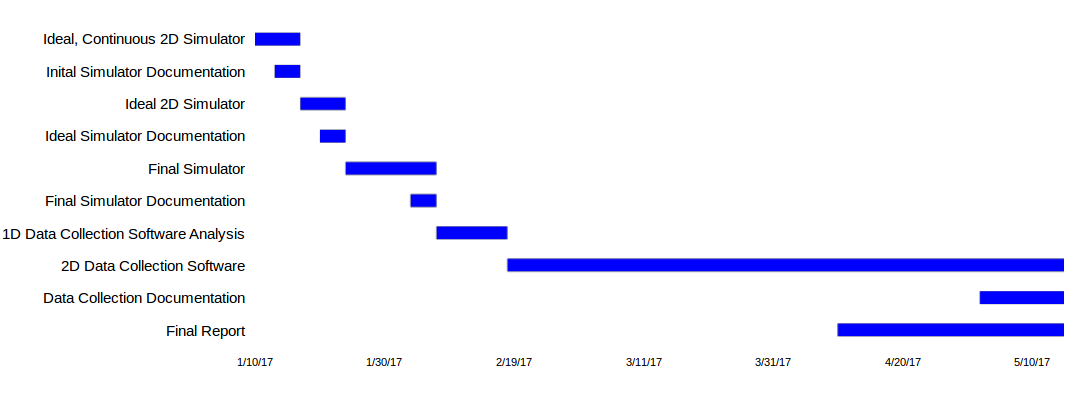
\includegraphics[width=1.2\textwidth]{timeline}
\caption{Project Timeline\label{chrt:time}}
\end{figure}

Labor cost estimates are
based on a rough \$44.00/hr starting pay for software engineers,
equivalent to \$440.00 per 7 days or about \$63.00/day, assuming I spend
10 hours week (standard part-time employment hours/week) working on these
tasks.

In short, the team requests \$15,189.50 to complete this project.
\section*{Conclusion}
The ability to reliably simulate 2D SPIFI systems is crucial to the ability
of the other teams working on the broader project to ensure the diffraction
patterns, wheel designs, and optical systems are correct implementations of
the theory, and are operating properly when placed into the system.
Furthermore, the entire point of performing SPIFI microscopy on an object
is to collect the output signal data, making the production of data
collection software imperative to the success of the project. The team
feels that costs have been estimated accurately, and that said costs are
well worth the advances to science this technology will bring.

Upon the project's completion, each of these software suites and their
corresponding source code will be made publicly available via a public
source control repository hosted by \href{http://www.gitlab.com}{GitLab}.
Specifically, both will be initiated as private repositories, but will be
made public upon publication of the larger body of work this team is
contributed to. As such, though links are provided in the Appendix,
following them will be useless to anyone without access to the
repositories, and will remain empty for a little while anyway. To request
access to these repositories, contact the project lead and/or head
software engineer. All links and contact information is available in
Appendix \ref{app:misc}.

\newpage
\section*{Appendix}
\appendix

\section{\label{app:misc}}
\subsection{Contact Information}
\begin{itemize}
\item Project Lead: Dr. Jeff Squire, \href{mailto:jsquier@mines.edu}{jsquier@mines.edu}
\item Team Head Software Engineer: Brennan W. Fieck, \href{mailto:bfieck@mymail.mines.edu}{bfieck@mines.edu}
\end{itemize}
\subsection{Links}
\begin{itemize}
\item \href{https://gitlab.com/PiercingGaze/2DSimulator}{2D SPIFI Grating Simulation Software}
\item \href{https://gitlab.com/PiercingGaze/SPIFIDataCollectionSoftware}{Data Collection Suite}
\item \href{https://www.researchgate.net/profile/Alyssa_Allende_Motz/publication/281058706_Super-resolved_multimodal_multiphoton_microscopy_with_spatial_frequency-modulated_imaging/links/5790535d08ae64311c0c7dbb.pdf?origin=publication_detail&ev=pub_int_prw_xdl&msrp=c3fj9RD45iTpvk8bRBlzYkN6ndcAYlW9SDWsP0gVb8WzFV5pplCJ3WT6D9fQrP2OT3rGfRWxpWECBz07rTxtH3ZWQ-V2CIIn99KlfPF-otY.9HgCklW2b18-KeSg_Y6vX11zOug1uQ3SSCEpbGXSzk5y_fIuZAdBHJtjk82L1NpfpV2e2Cvcd6QBkqBT24bFzQ.uEqPWNYXdN8Ge_jgkDmRdTlNB8rMwiFPPFdueuZQ9VY6c_KOsp-YvgMVBaNkL6Ldag5ifDVuL2YqcNGnICTcHA}{Original SPIFI Article} - hosted by
\href{https://www.researchgate.net}{Research Gate}
\end{itemize}
\newpage
\begin{thebibliography}{9}

\bibitem{lamport94}
  Squier, Dr Jeff. Deluca, Dr Keith. et. al.
  \emph{Super-Resolved Multimodal Multiphoton Microscopy with Spatial Frequency-Modulated
Imaging},
  Proceedings of the National Academy of Sciences,
  2015.
  
\bibitem{talk}
  Futia, Greg. Winters, Dave. Schlup, Philip. Bartels, Dr Randy.
  "Spatial Frequency Modulated Imaging on a Single Element Detector."
  Colorado School of Mines, Golden. May 24, 2011. Presentation.
  

\end{thebibliography}
\end{document}
